\documentclass[12pt]{article}
%^ Start of document
\usepackage{biblatex} %Imports biblatex package
\usepackage{graphicx} % Required for inserting images
\usepackage{authblk}
\usepackage[colorlinks=true, urlcolor=blue, linkcolor=red]{hyperref}
\usepackage{subfig}
\usepackage{float}
\usepackage{tabularx}
\usepackage{multirow}
\usepackage[paperheight=11in,
   paperwidth=8.5in,
   top=20mm,
   bottom=20mm,
   left=40mm,
   right=40mm]{geometry}
\usepackage{moresize}
\usepackage{tikz}
\usepackage{xcolor}
\usepackage{physics}
\usepackage{amssymb}
\usepackage{mathrsfs}
\usepackage{amsmath}
\usepackage{ragged2e}
\usepackage{comment}
\usepackage{xcolor}
\addbibresource{Electro.bib}
\begin{document}

\title{Classical Electrodynamics}

\author[1]{Zachary Tullier}
\affil[1]{Googler\\Anything you wanna know Department\\Houston, Texas\\U.S}

\maketitle

\begin{abstract}

\end{abstract}


\section{Old Math} \label{section1}

\subsection{Vectors} \label{subsection1-1}
    \begin{equation} \label{eq:1-1-1}
        a \cdot (b \cross c) = b \cdot (c \cross a) = c \cdot (a \cross b   
    \end{equation}
    \begin{equation} \label{eq:1-1-2}
        a \cross (b \cross c) = (a \cdot c) b - (a \cdot b) c
    \end{equation}
    \begin{equation} \label{eq:1-1-3}
        (a \cross b) \cdot (c \cross d) = (a \cdot c) (b \cdot d) - (a \cdot d) - (a \cdot d) (b \cdot c)
    \end{equation}
    \begin{equation} \label{eq:1-1-4}
        \nabla \cross \nabla \psi = 0
    \end{equation}
    \begin{equation} \label{eq:1-1-5}
        \nabla \cdot (\nabla \cross a) = 0
    \end{equation}
    \begin{equation} \label{eq:1-1-6}
        \nabla \cross (\nabla \cross a) = \nabla (\nabla \cdot a) - \nabla^2 a 
    \end{equation}
    \begin{equation} \label{eq:1-1-7}
        \nabla \cdot (\psi a) = a \cdot \nabla \psi + \psi \nabla \cdot a
    \end{equation}
    \begin{equation} \label{eq:1-1-8}
        \nabla \cross (\psi a) = \nabla psi \cross a + \psi \nabla \cross a 
    \end{equation}
    \begin{equation} \label{eq:1-1-9}
        \nabla (a \cdot b) = (a cdot \nabla) b + (b \cdot \nabla) a + a \cross (\nabla \cross b) + b \cross (\nabla \cross a)
    \end{equation}
    \begin{equation} \label{eq:1-1-10}
        \nabla \cdot (a \cross b) = b \cdot (\nabla \cross a) - a \cdot (\nabla \cross b)
    \end{equation}
    \begin{equation} \label{eq:1-1-11}
        \nabla \cross (a \cross b) = a (\nabla \cdot b) - b (\nabla \cdot a) + (b \cdot \nabla) a - (a \cdot \nabla) b
    \end{equation}
    Divergence Theorem
    \begin{equation} \label{eq: 1-1-12}
        \int_V \nabla \cdot A d^3x = \int_S A \cdot n da
    \end{equation}
    \begin{equation} \label{eq: 1-1-13}
        \int_V \nabla \psi d^3x = \int_S \psi n da
    \end{equation}
    \begin{equation} \label{eq: 1-1-14}
        \int_V \nabla \cross A d^3x = \int_S n \cross A da
    \end{equation}
    Green's first Identity
    \begin{equation} \label{eq: 1-1-15}
        \int_V (\phi \nabla^2 \psi + \nabla \phi \cdot \nabla \psi) d^3x = \int_S \phi n \cdot \nabla \psi da
    \end{equation}
    Greens Theorem
    \begin{equation} \label{eq: 1-1-16}
        \int_V (\phi \nabla^2 \psi - \psi \nabla^2 \phi) d^3x = \int_S (\phi \nabla \psi - \psi \nabla \phi) \cdot n da
    \end{equation}
    Stoke's Theorem
    \begin{equation} \label{eq: 1-1-17}
        \int_S (\nabla \cross A) \cdot da = \oint_C A \cdot dl
    \end{equation}
    \begin{equation} \label{eq: 1-1-18}
        \int_S n \cross \nabla \psi da = \oint_C \psi dl
    \end{equation}
    $C$ is the contour bounding the Open Surface $S$ with $dl$ as the line element of the contour
\begin{figure}[H]
    \centering
    \subfloat[Vector Formulas]{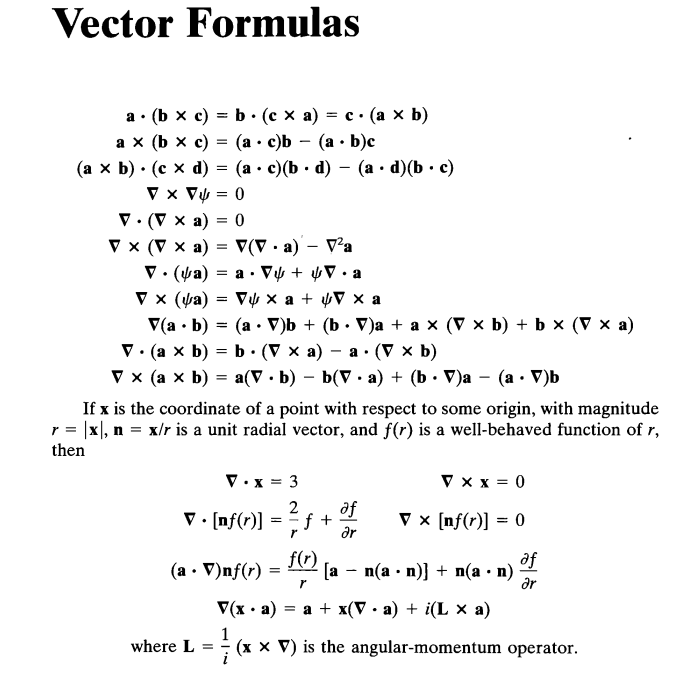
\includegraphics[width=0.5\textwidth]{Images/Vector Formulas.PNG}\label{fig:f1}}
    \hfill
    \subfloat[Vector Theorems]{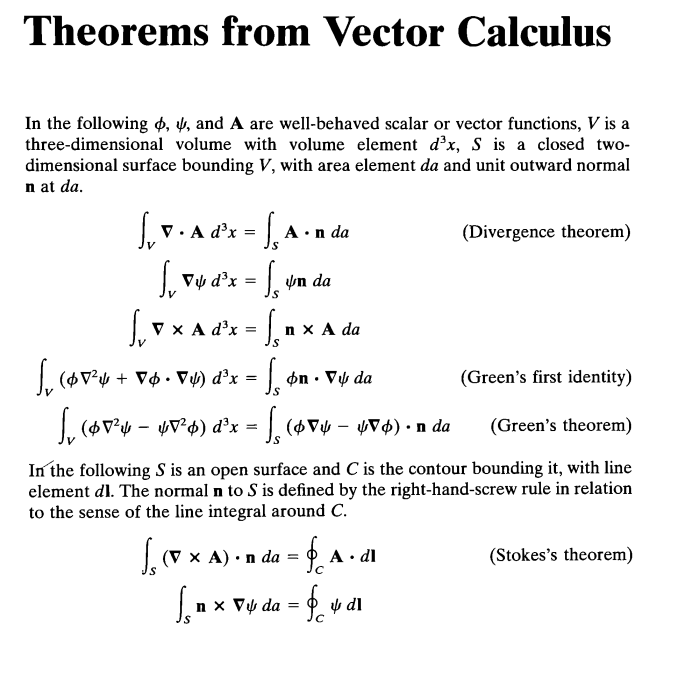
\includegraphics[width=0.5\textwidth]{Images/Vector Theorems.PNG}\label{fig:f2}}
\end{figure}
 $\hat{r} = \frac{\vec{r}}{\abs{r}}$
%\newline \textcolor{red}{What does $\hat{r}$ stand for?. Is this equation correct?}
\newline On page \pageref{eq:1-1-1} equation \ref{eq:1-1-1}

\subsection{Dirac Delta Properties} \label{subsection1-2}
    Where the prime is differentiation with respect to the argument.
    %\newline \textcolor{red}{Don't understand above statement}
    \begin{equation} \label{eq: 1-2-1}
        \delta(x-a) = a  \mbox{ for } x \neq a
    \end{equation}
    if the region of integration includes x=a
    \begin{equation} \label{eq: 1-2-2}
        \int \delta(x-a)dx = 1 
    \end{equation}
    and is zero otherwise  ($x \neq a$)
    \begin{equation} \label{eq: 1-2-3}
        \int \delta(x-a)dx = 0
    \end{equation}
    \begin{equation} \label{eq: 1-2-4}
        \int f(x) \delta(x-a) dx = f(a)
    \end{equation}
    \begin{equation} \label{eq: 1-2-5}
        \int f(x) \delta^{'}(x-a)dx = -f^{'}(a)
    \end{equation}
    \begin{equation} \label{eq: 1-2-6}
        \delta(f(x)) = \sum \frac{1}{\frac{df}{dx}x_i} \delta(x-x_i)
    \end{equation}
    \begin{equation} \label{eq: 1-2-7}
        \delta^{(3)}=U \delta(x-x_o) V \delta(y-y_0) W \delta(z-z_0)
    \end{equation}
    If $\Delta V$ contains $x=X$
    \begin{equation} \label{eq: 1-2-8}
        \int_{\Delta V} \delta(x-X) d^3 x = 1
    \end{equation}
    If $\Delta V$ does not contain $x=X$
    \begin{equation} \label{eq: 1-2-9}
        \int_{\Delta V} \delta(x-X) d^3 x = 0
    \end{equation}
    \begin{equation} \label{eq: 1-2-10}
        \delta(au)=\frac{1}{\abs{a}} \delta(u)
    \end{equation}

\subsection{Various Old Math} \label{section1-3}
    The 3D volume element at $dx'$
    \begin{equation} \label{eq: 1-3-1}
        d^3x' = dx' dy' dz'    
    \end{equation}
    

\section{New Math} \label{section2}
    \begin{equation} \label{eq: 2-1}
        \rho_q = q_i \delta^{(3)} (x-x_i)    
    \end{equation}
    \begin{equation} \label{eq: 2-2}
        \rho_\lambda = \lambda_i \delta^{(2)}     
    \end{equation}
    \begin{equation} \label{eq: 2-3}
        \rho_\sigma = \sigma_i \delta^{(1)}     
    \end{equation}

\section{Electrodynamics} \label{section3}

\subsection{Putting charge at origin} \label{subsection3-1}
    Using general 3D Dirac Delta function (Reference equ \ref{eq: 1-2-7} on pg \pageref{eq: 1-2-7})
    \newline $\delta^{(3)}=U \delta(x-x_o) V \delta(y-y_0) W \delta(z-z_0)$
    \newline Replace Cartesian with spherical coordinates ($r, \theta, phi)$ 
    \newline Modify $U,V,W$ with incremental length elements ($dr, rd\theta, r sin(theta) d\phi)$
    %\newline \textcolor{red}{Don't understand in between}
    \newline This makes $U = 1, V = \frac{1}{r}, W = \frac{1}{r sin(\theta)}$
    \begin{equation} \label{eq: 3-1-1}
        \delta^{(3)} = \delta(r-r_0) \frac{\delta (\theta - \theta_0)}{r} \frac{\delta (\phi - \phi_0)}{r sin(\theta)}
    \end{equation}
    \newline For 2D data in spherical coordinates we consider a circular 2D ring with a radius of $R$, lying in the x-y plane. This makes $r_0 = R$, $\theta_0 = \frac{\pi}{2}$, and $\phi-\phi_0 = 0$
    \begin{equation} \label{eq: 3-1-2}
        \delta^{(2)}_{ring} = \delta(r-R) \frac{\delta(\theta - \frac{\pi}{2})}{r}
    \end{equation}
    \newline For thin spherical shell. This makes $r_0 = R$, $\theta - \theta_0 = 0$, and $\phi-\phi_0 = 0$
    \begin{equation} \label{eq: 3-1-3}
        \delta^{(1)}_{shell} = \delta(r-R)
    \end{equation}
    \newline For point charge at origin in spherical coordinate
    \begin{equation} \label{eq: 3-1-4}
        \delta^{(3)}_{origin} = \frac{\delta(r)}{4 \pi r^2}
    \end{equation}
    %\newline \textcolor{red}{Don't understand in between}
    \begin{equation} \label{eq: 3-1-5}
        \vec{E} = k \frac{q}{r^{2}} \hat{r}
    \end{equation}
    %\newline \textcolor{red}{Where did the above come from?}
    \newline For line charge along z axis of cylindrical coordinates
    \begin{equation} \label{eq: 3-1-6}
        \delta^{(2)}_{cylLine} = \frac{\delta(\rho)}{2 \pi \rho}
    \end{equation}
    %\newline \textcolor{red}{Don't understand in between}

\subsection{Coulomb's Law} \label{subsection3-2}
    Two Electric point charges exert a force on each other.
    \begin{equation} \label{eq: 3-2-1}
        \vec{F} = q \vec{E} = k q_1 q_2 \frac{x_1-x_2}{\abs{x_1-x_2}^3}
    \end{equation}
    \newline Electric field at point x due to a point charge
    \begin{equation} \label{eq: 3-2-2}
        \vec{E} = k q_1 \frac{x-x_1}{\abs{x-x_1}^3}
    \end{equation}
    \newline In electrostatic units (esu) k = 1, In SI:
    \begin{equation} \label{eq: 3-2-3}
        k = \frac{1}{4 \pi \epsilon_0} = 10^{-7} c^2
    \end{equation}
    \newline Since Electrodynamics is a macroscopic theory, we will consider the "point" to be many charged sources. Experiment shows that the fields add linearly.
    \begin{equation} \label{eq: 3-2-4}
        \vec{E}(x)= k \sum_i q_i \frac{x-x_i}{\abs{x - x_i}^3}
    \end{equation}
    \newline Consider the many charged sources to be "small" (Replace $q$ with $\rho$) and "numerous" (Replace Sum with Integral)at point $x'$. Coulomb's law in terms of the field for a charge density. Replace singular x dimension with 3D x,y,z dimension (Reference \ref{eq: 1-3-1} on pg \pageref{eq: 1-3-1})
    \begin{equation} \label{eq: 3-2-5}
        \vec{E}(x)= k \int \rho_q(x') \frac{x-x'}{\abs{x - x'}^3}d^3x'
    \end{equation}
    \newline Replacing point charge density with sheet charge density (Reference \ref{eq: 2-2} on pg \pageref{eq: 2-2} we get coulomb's integral form for the electric field at point x due to a sheet charge
    \begin{equation} \label{eq: 3-2-6}
        \vec{E}(x)= k \int \sigma(x') \frac{x-x'}{\abs{x - x'}^3}d^3x'
    \end{equation}
    \newline Replacing point charge density with line charge density (Reference \ref{eq: 2-3} on pg \pageref{eq: 2-3} we get coulomb's integral form for the electric field at point x due to a line charge
    \begin{equation} \label{eq: 3-2-7}
        \vec{E}(x)= k \int \lambda(x') \frac{x-x'}{\abs{x - x'}^3}d^3x'
    \end{equation}
    \newline The following is proof of the previous formulation
    \newline Describe charge density using Dirac Delta function properties (Reference \ref{eq: 2-1} on pg \pageref{eq: 2-1}
    \begin{equation} \label{eq: 3-2-8}
        \vec{E}(x)= k \int \sum q_i \delta(x - x_i) \frac{x-x'}{\abs{x - x'}^3}d^3x'
    \end{equation}
    \newline After Integration this verifies our earlier assumption (Reference equ \ref{eq: 3-2-2} on pg \pageref{eq: 3-2-2})
    \begin{gather*}
        \vec{E} = k q_1 \frac{x-x_1}{\abs{x-x_1}^3}
    \end{gather*}
    \newline Coulomb's Law does not include bounding surfaces. Therefore the integral must be done over all charges in the universe, or we must assume that most of the charges in the universe are far enough away that their contribution is negligible. Because of this fact, Coulomb's law has limited applicability. 

\subsection{Gauss Law} \label{subsection3-3}
    \begin{figure}[H]
        \centering
        \subfloat[Gauss Law Formula Variables]{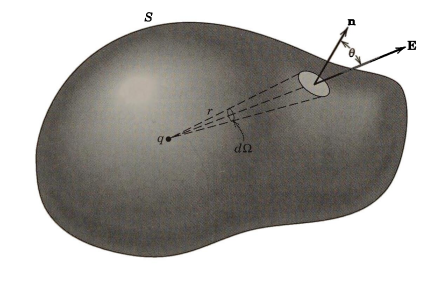
\includegraphics[width=0.5\textwidth]{Images/GaussLaw.PNG}\label{fig:f1}}
    \end{figure}
    Take Coulomb's law for a point charge (Ref equ \ref{eq: 3-2-2} on pg \pageref{eq: 3-2-2})
    \begin{gather*}
        \vec{E}(x) = k q \frac{x-x_1}{\abs{x-x_1}^3}
    \end{gather*}
    \newline As before, put the charge at the origin (Ref equ \ref{eq: 3-1-5} on pg \pageref{eq: 3-1-5})
    \begin{gather*}
        \vec{E} = k \frac{q}{r^2} \hat{r}
    \end{gather*}
    \newline Dot both sides by the normal vector 
    \begin{equation}
        \vec{E} = k \frac{q}{r^2} cos(\theta)    
    \end{equation}
    \newline Integrate both sides over the closed surface
    \begin{equation}
        \oint_S (\vec{E} \cdot n) da = \oint_S (k \frac{q}{r^2} cos(\theta)) da
    \end{equation}
    \newline Since E is directed along the line from surface element to the charge q
    \begin{equation}
        \oint_S (\vec{E} \cdot n) da = \oint_S (k \frac{q}{r^2} r^2) d\Omega
    \end{equation}
    \newline Simple algebra eliminates $r^2$, and take constants out of integral 
    \begin{equation}
        \oint_S (\vec{E} \cdot n) da = k q \oint_S d\Omega
    \end{equation}
    \newline Expand k (Ref equ \ref{eq: 3-2-3} on pg \pageref{eq: 3-2-3})
    \begin{equation}
        \oint_S (\vec{E} \cdot n) da = \frac{q}{4 \pi \epsilon_0} \oint_S d\Omega
    \end{equation}
    \newline Integrate $\Theta$ to get total charge enclosed by Gaussian surface. 
    \begin{equation}
        \oint_S d\Theta = \int_0^{2 \pi} \int_0^\pi d\Theta
    \end{equation}
    \newline Replace $\Theta$ with cylindrical coordinates (Ref fig \ref{fig:f1} on pg \ref{fig:f1}
    \begin{equation}
        \oint_S d\Theta = \int_0^{2 \pi} \int_0^\pi r^2 sin(\theta) d \theta d \phi = 4 \pi
    \end{equation}
    \newline Place Integration back into equation (Ref equ \ref{} on pg \pageref{})
    \begin{equation}
        \oint_S (\vec{E} \cdot n) da = \frac{4 q \pi}{4 \pi \epsilon_0} = \frac{q}{\epsilon_0}
    \end{equation}
    \newline The above equation is true for any charge completely enclosed by Gaussian surface. For any charge outside of Gaussian surface:
    \begin{equation}
        \oint_S \vec{E} \cdot n da = 0
    \end{equation}
    \newline For a discrete set of charges 
    \begin{equation}
        \oint_S \vec{E} \cdot n da = \frac{\sum q_i}{\epsilon_0}
    \end{equation}
    \newline For continuous charge density
    \begin{equation}
        \boxed{\boldsymbol{\oint_S \vec{E} \cdot n da = \frac{\int_V \rho_q(x) d^3 x}{\epsilon_0}}}
    \end{equation}
    \newline Apply Divergence Theorem (Ref equ \ref{eq: 1-1-12} on pg \pageref{eq: 1-1-12})
    \begin{equation}
        \int_V \nabla \cdot \vec{E} d^3 x = \frac{\int_V \rho_q(x) d^3 x}{\epsilon_0}
    \end{equation}
    \newline Apply simple algebra to get Gauss's Law in differential form
    \begin{equation}
        \int_V (\nabla \cdot \vec{E} - \frac{\rho_q(x)}{\epsilon_0}) d^3 x = 0
    \end{equation}
    \begin{equation}
        \boxed{\boldsymbol{\nabla \cdot \vec{E}= \frac{\rho_q(x)}{\epsilon_0}}}
    \end{equation}
    \newline In comparison to Coulomb's Law and Gauss's law in integral form, Gauss's differential equation is local and therefore most useful in practice. 
    \newline For the very specific case of the electric field being constant across the surface and everywhere perpendicular to the surface
    %\newline \textcolor{red}{Do in between math work. Shouldn't this be dot product}
    \begin{equation}
        \vec{E} = E_0 n
    \end{equation}
    \begin{equation}
        E_0 \oint_S da = \frac{\int_V \rho_q(x) d^3 x}{\epsilon_0}
    \end{equation}
    \begin{equation}
        E_0 A_S = \frac{\int_V \rho_q(x) d^3 x}{\epsilon_0}
    \end{equation}
    \begin{equation}
        E_0= \frac{\int_V \rho_q(x) d^3 x}{\epsilon_0 A_S}
    \end{equation}

\subsection{Scalar Potential} \label{section3-4}
    A vector field can be specified completely if its divergence and curl are given everywhere in space, except up to the gradient of scalar function that satisfies the Laplace equation. 
    %\newline \textcolor{red}{when you get to section 1.9, this Laplace stuff might come into play}
    \newline Therefore we need to specify the curl of $\vec{E}$
    \newline Starting at Coulomb's generalized integral form (Reference equation \ref{eq: 3-2-5} on page \pageref{eq: 3-2-5}
    \begin{gather*}
        \vec{E(x)}= k \int \rho_q(x^{'}) \frac{x-x^{'}}{\abs{x - x'}^3}d^3x'
    \end{gather*}
    %\newline \textcolor{red}{I guess I don't know how $\nabla$ works. Figure out in between}
    \newline Using Property of Nabla ($\nabla$)
    \begin{equation} \label{eq: 3-4-1}
        -\nabla(\frac{1}{\abs{x-x'}}) = \frac{x-x'}{\abs{x - x'}^3}
    \end{equation}
    Substitute equation \ref{eq: 3-4-1} into \ref{eq: 3-2-5}
    \begin{equation} \label{eq: 3-4-2}
        \vec{E(x)}= k \int \rho_q(x') -\nabla(\frac{1}{\abs{x-x'}}d^3x'
    \end{equation}
    Nabla ($\nabla$) is constant; therefore,
    \begin{equation} \label{eq: 3-4-3}
        \vec{E(x)}= -k \nabla \int \rho_q(x') (\frac{1}{\abs{x-x'}}d^3x'
    \end{equation}
    Cross nabla ($\nabla$) on both sides of equation and substitute equation \ref{eq:1-1-4} 
    \begin{equation} \label{eq: 3-4-4}
        \nabla \cross \vec{E(x)}= \nabla \cross k -k\nabla \int \rho_q(x') (\frac{1}{\abs{x-x'}}d^3x'
    \end{equation}
    Therefore,
    \begin{equation} \label{eq: 3-4-5}
        \nabla \cross \vec{E} = 0
    \end{equation}
    By manipulating equation \ref{eq: 3-4-3}
    \begin{equation} \label{eq: 3-4-6}
        \vec{E(x)}= \nabla \int (\frac{k \rho_q (x')}{\abs{x-x'}}d^3x'
    \end{equation}
    We can now define a portion of the equation as the scalar potential ($\Phi$)
    \begin{equation} \label{eq: 3-4-7}
        \vec{E(x)}= \nabla \Phi
    \end{equation}
    Work done can be defined as moving a charge from point A to point B in an electric field
    \begin{equation} \label{eq: 3-4-8}
        W = - \int_A^B \vec{F} \cdot dx
    \end{equation}
    %\textcolor{red}{the book and the notes use L instead of x. It is noting that there is a path between point A and B and dL is some small length of that path. I hate that, so I put x}
\newline Substitute equation \ref{eq: 3-2-1} into 
\newline $W = -q \int_A^B \vec{E} \cdot dx $
\newline Substitute from previously formulated equ
\newline $W = q \int_A^B \nabla \Phi \cdot dx$
%\newline \textcolor{red}{Don't know this in between, maybe vector def}
\newline $W = q \int_A^B d\Phi$
\newline Integrate
\newline $W = q (\Phi_B - \Phi_A)$
\newline By work-energy theorem, work and energy are equivalent, therefore
\newline $\Delta \Phi = \frac{U}{q}$
\newline Substitute previously formulated
\newline $-q\int_A^B \vec{E} \cdot dx = q (\Phi_B - \Phi_A)$
\newline if path is closed
\newline $\oint \vec{E} \cdot dx = 0$
%\newline \textcolor{red}{Section 1.6 is partially covered in notes. Come back to section 1.6 and 1.7 if you have time.}

\subsection{Capacitance}
Collection of separate objects that are perfect conductors residing in free space. The charge, conductor potentials and geometric properties are the only links to the free space and the conductors. 
\newline The electrostatic potential at any point in space due to a collection of $n$ objects is just the sum of all individual potentials
\newline $\Phi = k \sum \int \frac{\rho_j(x^{'}}{\abs{x-x^{'}}} dx^{'}$
\newline We only care about points in space on the surface of the objects, so $x_i$ is a point on the surface of i object
\newline $\Phi(x_i) = k \sum \int \frac{\rho_j(x^{'}}{\abs{x_i-x^{'}}} dx^{'}$
%\newline \textcolor{red}{The book uses the variable $V_i$ to represent the electrostatic potential of each conductor when they are a constant value. Calling it equipotential. I don't like this so I am going to use $\Phi(x_i)$ instead.}
\newline Since normalized charge density $\frac{\rho_j(x^{'}}{Q_j}$ is purely geometrical, where $Q_j$ is the total charge on the plate we can do the following. This is an approximation/assumption because the charge density "tends" to spread out into the same minimal energy pattern when a charge is applied. 
\newline $\Phi(x_i) = k \sum_j \int \frac{\rho_j(x^{'} Q_j}{\abs{x_i-x^{'}}Q_j} dx^{'}$
\newline Simple algebra and removing $Q_j$ from the integral
\newline $\Phi(x_i) = \sum Q_j k \int \frac{\rho_j(x^{'}}{\abs{x_i-x^{'}}Q_j} dx^{'}$
\newline We now define the Geometric Coefficient $p_{ij}$ which is the normalized electric potential felt at the $i^{th}$ conductor due to the $j^{th}$ conductor. 
\newline $p_{ij} = k \int \frac{\rho_j(x^{'}}{\abs{x_i-x^{'}}Q_j} dx^{'}$
\newline $\Phi(x_i) = \sum p_{ij} Q_j$
\newline Invert equation for more practical use
\newline $Q_i = \sum p_{ij} \Phi_j$
\newline We now define the generalized Geometric Coefficient as Capacitance $C$
\newline $Q_i = \sum C_{ij} \Phi_j$
\newline For 2 conductors, we have
\newline $Q_1 = C_11 \Phi_1 + C_12 \Phi_2$
\newline $Q_2 = C_21 \Phi_1 + C_22 \Phi_2$
%\newline \textcolor{red}{They did some funky math here and said "subtract $\Phi_2$ from each potential to get rid of the second term". Then wrote the following}
\newline $Q_1 = C_11 (\Phi_1 - \Phi_2)$
\newline Algebra
\newline $C_11 = \frac{Q_1}{\Phi_1 - \Phi_2}$
\newline $C = \frac{Q}{\Delta \Phi}$
\newline $\Delta \Phi$ is the difference in electrostatic potential which is commonly referred to as voltage ($V$), so
\newline $C = \frac{Q}{\Delta V}$

\subsection{Surface Charge Density}
Take Gauss's Law in integral form
\newline $\oint_S \vec{E} \cdot n da = \frac{\int_V \rho_q(x) d^3 x}{\epsilon_0}$
\newline Take this integral in the form of a charged sheet
\newline $\oint_S \vec{E} \cdot n da = \frac{\int_V \rho_sigma(x) d^3 x}{\epsilon_0}$
\newline With out definition of $\rho_sigma$ in terms of Dirac Delta function
\newline $\oint_S \vec{E} \cdot n da = \frac{\int_V \sigma \delta (n^{'}-n_0^{'} d^3 x}{\epsilon_0}$
\newline where $n^{'}$ is the position vector normal to the surface and $n_0^{'}$ is the location on that vector that meets the surface. 
\newline The top, bottom and "thickness" are considered. The "thickness" cancels itself out because it is a loop parallel to the electric fields. The volume chosen is small enough that the surfaces are considered flat; therefore, $n=n^{'}$ on the top tide and $n=n^{'}$ on the bottom. 
\newline $\oint_S \vec{E_2} \cdot n^{'} d^2 x - \oint_S \vec{E_1} \cdot n^{'} d^2x= \frac{\int_V \sigma \delta (n^{'}-n_0^{'} d^3 x}{\epsilon_0}$
%\newline \textcolor{red}{How did $da$ become $d^2 x$}
\newline If the area is chosen small enough then the sheet would not experience different electric fields in different locations
\newline $\vec{E_2} \cdot n^{'} \oint_S d^2x - \vec{E_1} \cdot n^{'} \oint_S d^2x = \frac{\int_V \sigma \delta (n^{'}-n_0^{'} d^3 x}
{\epsilon_0}$
\newline The surface charge density ($\sigma$) is "distributed" so it can be taken out of integral
\newline $\vec{E_2} \cdot n^{'} \oint_S d^2x - \vec{E_1} \cdot n^{'} \oint_S d^2x = \frac{\sigma}{\epsilon_0} \int_V \delta (n^{'}-n_0^{'} d^3x$
%\newline \textcolor{red}{IDK why this next part is, but it is the "common variable" method in math where you can just get rid of stuff. Maybe its by turning the volumetric integral into a point integral. Also, how do $\oint_S$ and $\int_V$ compare in this situation}
\newline $\vec{E_2} \cdot n^{'} \oint_S d^2x - \vec{E_1} \cdot n^{'} \oint_S d^2x = \frac{\sigma}{\epsilon_0} \int_S d^2x \int_V \delta (n^{'}-n_0^{'} d^x$
\newline Get ride of all $\int_S d^2x$
\newline $\vec{E_2} \cdot n^{'} - \vec{E_1} \cdot n^{'} = \frac{\sigma}{\epsilon_0} \int_V \delta (n^{'}-n_0^{'} d^x$
\newline Take integral, but $n^{'} = n_0^{'}$
\newline $\boxed{\boldsymbol{(\vec{E_2} - \vec{E_1}) \cdot n^{'} = \frac{\sigma}{\epsilon_0}}}$
%\newline \textcolor{red}{Notes say to "Master" this derivation}
\newline This equation is called "Surface Charge Density of an Arbitrary Surface. It can be used for the following
\begin{itemize}
    \item To find the surface charge density if we know the fields
    \item To connect two regions at their boundary if we know the fields in both regions up to a constant
    \item To find the fields everywhere if we know the surface charge density and the geometry
\end{itemize}
For case 2
\newline As seen before. Electrostatic fields are irrotational
%\newline \textcolor{red}{Where is before}
\newline $\nabla \cross \vec{E} = 0$
\newline Integrate over some arbitrary open surface
\newline $\int (\nabla \cross \vec{E}) \cdot n da = 0$
\newline Use Stoke's theorem to convert this to a closed line integral around the edge of the surface
%\newline \textcolor{red}{Practice this in between stokes theorem}
\newline $\oint \vec{E \cdot dx = 0}$
%\newline \textcolor{red}{The notes use $l$ instead of $x$. I hate this notation}
\newline The above is the integral form of the statement "Electrostatic fields are irrotational"
\newline Take the integral over a rectangular closed loop $\textbf{that straddles the boundary surface}$. Not a surface. 
\begin{figure}[H]
    \centering
    \subfloat[Closed loop straddling the boundary surface]{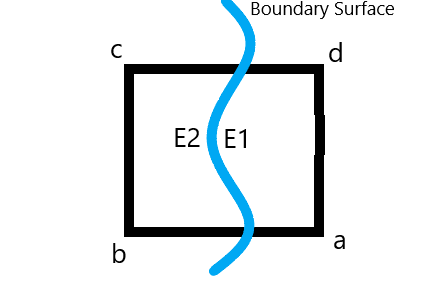
\includegraphics[width=0.5\textwidth]{Images/ClosedLoopStraddleSurface.png}\label{fig:f1}}
\end{figure}
%\textcolor{red}{Make this make sense. Cant get the image down}
\newline $\int_a^b \vec{E_1} \cdot dx + \int_b^a \vec{E_2} \cdot dx = 0$
\newline Electric field is constant along length of loop
\newline $\vec{E_1} \cdot \int_a^b dx + \vec{E_2} \cdot \int_b^a dx = 0$
\newline change direction of integral to equate
\newline $\vec{E_1} \cdot \int_a^b dx - \vec{E_2} \cdot \int_a^b dx = 0$
%\newline \textcolor{red}{Do integral?}
\newline $E_1 = E_2$
\newline We will call them tangential components of electric field ($E_{1,T}$ and $E_{2,T}$)
\newline $\boxed{\boldsymbol{\vec{E_1} \cross n = \vec{E_2} \cross n}}$

\subsection{Maxwell's Boundary Conditions}
There should be six conditions
\begin{gather*}
    Surface Charge Density on an Arbitrary Surface
    \\ \boxed{\boldsymbol{(\vec{E_2} - \vec{E_1}) \cdot n^{'} = \frac{\sigma}{\epsilon_0}}}
    The components of the electric field that are tangential to a surface are continuous across the surface even if a surface charge density is present
    \\\boxed{\boldsymbol{\vec{E_1} \cross n = \vec{E_2} \cross n}}
    \\
\end{gather*}

\subsection{Greens Functions}
Coulomb's Law can be transformed to include boundary conditions instead of an integral over the whole universe through the use of mathematical tools called Green functions
\newline Greens functions are applications of the divergence theorem
\newline $\int_V \nabla \cdot A d^3x = \int_S A \cdot da$
\newline $A$ is an arbitrary vector field. Define $A = \phi \nabla \Psi$, where $\phi$ and $\Psi$ are arbitrary scalars
%\newline \textcolor{red}{Need to know more about $\nabla$ to be able to describe the above definition}
%\newline \textcolor{red}{The notes use $^{'}$ alot, but I don't like it.}
\newline $\int_V \nabla \cdot \phi \nabla \Psi d^3x = \int_S \phi \nabla \Psi \cdot da$
\newline Use property of dot product
%\newline \textcolor{red}{Need to learn properties of dot product}
\newline $\int_V \nabla \phi \cdot \nabla \Psi + \phi \nabla^2 \Psi d^3x = \int_S \phi \frac{d\Phi}{dn} da$
\newline Interchange scalars and subtract the two equations
\newline $\int_V \nabla \phi \cdot \nabla \Psi - \nabla \Psi \cdot \nabla \phi + \phi \nabla^2 \Psi - \Psi \nabla^2 \phi d^3x = \int_S \phi \frac{d\Psi}{dn} - \Psi \frac{d\phi}{dn} da$
\newline Simplify
\newline $\int_V \phi \nabla^2 \Psi - \Psi \nabla^2 \phi d^3x = \int_S \phi \frac{d\Psi}{dn} - \Psi \frac{d\phi}{dn} da$
%\newline \textcolor{red}{Again, Need to learn properties of dot product to know why $\nabla \phi \cdot \nabla \Psi - \nabla \Psi \cdot \nabla \phi = 0$}
\newline Assign $\phi = \Phi$ and $\Psi = G(x,x^{'}) = \frac{1}{\abs{x-x^{'}}}+F(x,x^{'})$
\newline $\int_V \Phi \nabla^2 G(x,x^{'} - G(x,x^{'} \nabla^2 \Phi d^3x = \int_S \Phi \frac{dG(x,x^{'}}{dn} - G(x,x^{'} \frac{d\Phi}{dn} da$
\newline Require that $\nabla^2 F(x,x^{'}) = 0$
\newline $\nabla^2 G(x,x^{'}) = \nabla^2 \frac{1}{\abs{x-x^{'}}}$
\newline Use Identity $\nabla^2 \frac{1}{\abs{x-x^{'}}} = -4 \pi \delta(x-x^{'}$
%\newline \textcolor{red}{No clue where this identity comes from}
\newline $\int_V \Phi (-4 \pi \delta(x-x^{'}) - G(x,x^{'} \nabla^2 \Phi d^3x = \int_S \Phi \frac{dG(x,x^{'}}{dn} - G(x,x^{'} \frac{d\Phi}{dn} da$
\newline Use Poisson's Equation and Evaluate the integral
%\newline \textcolor{red}{How to use Poissons Equation}
\newline $-4 \pi \Phi(x) + \frac{\int \rho(x^{'} G d^3x}{\epsilon_0} = \int_S \Phi \frac{dG(x,x^{'}}{dn} - G(x,x^{'} \frac{d\Phi}{dn} da$
\newline Isolate Scalar potential ($\Phi(x)$)
\newline $\Phi(x) = \frac{\int \rho(x^{'} G d^3x}{4 \pi \epsilon_0} + \frac{\int_S \Phi \frac{dG(x,x^{'}}{dn} - G(x,x^{'} \frac{d\Phi}{dn} da}{4 \pi}$
\newline This is the Green function solution to the electrostatic equations
\newline This practically converts an "integral over all space" into a "integral over a limited volume" plus a correction term. 
\newline The "Correction term" $\frac{\int \rho(x^{'} G d^3x}{4 \pi \epsilon_0}$ is the integral of the boundary conditions over the surface enclosing the volume
%\newline \textcolor{red}{Not sure if I got the right side of the equation as the "Correction term"}
\newline The Green Function ($G$) is the weighting parameter and it is problem dependent. We must find the right function F that makes one of the last two terms vanish. 
\newline For Dirichlet boundary condition ($\Phi(x^{'}$ is known on the surface of integration), we assign $G = 0$
\newline $\Phi(x) = \frac{\int \rho(x^{'} G d^3x}{4 \pi \epsilon_0} + \frac{\int_S \Phi \frac{dG}{dn} da}{4 \pi}$
%\newline \textcolor{red}{Dive deeper. Book should have more on Dirichlet boundary condition}
\newline for Neumann boundary condition ($\frac{\Phi(x^{'}}{dn}$ is known on the surface of integration) we assign $\frac{dG}{dn} = \frac{-4 \pi}{S}$ where S is the total surface area
\newline $\Phi(x) = \frac{\int \rho(x^{'} G d^3x}{4 \pi \epsilon_0} + \frac{\int_S G \frac{d\Phi}{dn} da}{4 \pi} + \textlangle \Phi \textrangle_S $
\newline if the surface is infinite than $\textlangle \Phi \textrangle_S = 0$
%\newline \textcolor{red}{Dive deeper. Book should have more on Neumann boundary condition}
\newline We learn later how to find the right green function

\subsection{Energy Density}
Previously Formulated
\newline $W = q (\Phi_B - \Phi_A)$
\newline Test point charge is brought in from infinity making $\Phi_A = 0$
\newline $W = q (\Phi)$
\newline expanding $\Phi$
\newline $w = q k \int \frac{\rho(x^{'})}{\abs{x-x^{'}}} dx^{'}$
%\newline \textcolor{red}{Again, don't understand $^{'}$}
\newline Expanding k
\newline $w = \frac{q}{4 \pi \epsilon_0} \int \frac{\rho(x^{'})}{\abs{x-x^{'}}} dx^{'}$
\newline Bring multiple charges in from infinity, one at a time
%\newline \textcolor{red}{I think this is just addition, workout}
\newline $w = \frac{q}{8 \pi \epsilon_0} \int \int \frac{\rho(x) \rho(x^{'})}{\abs{x-x^{'}}} dx dx^{'}$
\newline Using Coulomb's Law and the Poissons Equation
%\newline \textcolor{red}{need lots of in between steps}
\newline $-\frac{\epsilon_0}{2} \int \Phi \nabla^2 \Phi dx$
\newline Integration by parts
%\newline \textcolor{red}{need lots of in between steps}
\newline $\frac{\epsilon_0}{2} \int \abs{\nabla \Phi}^2 dx$
\newline previously formulated
\newline $\frac{\epsilon_0}{2} \int \abs{\vec{E}}^2 dx$
\newline $\vec{E}$ is not dependent on x 
\newline $\frac{\abs{\vec{E}}^2 \epsilon_0}{2}$

\subsection{Point Charge in the Presence of a Grounded Sphere} \label{sectionPC}
    $y$ as the distance to point charge from the origin, $y'$ as the distance to the image charge from the origin, and $a$ as radius of sphere as shown in figure
    \begin{figure}[H]
        \centering
        \subfloat[Point charge outside of a charged sphere with a charge "image" on the inside of the sphere]{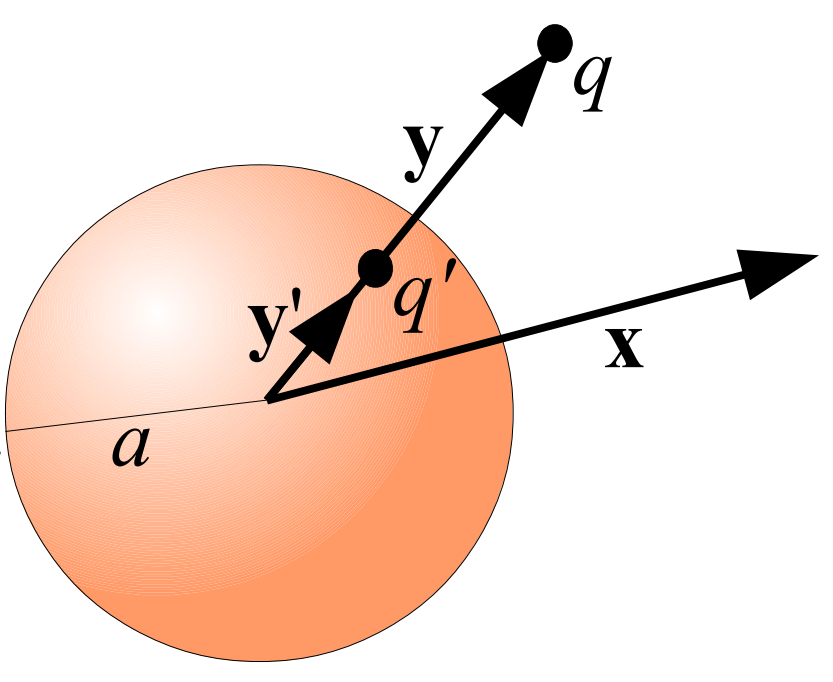
\includegraphics[width=0.5\textwidth]{Images/ImageCharge.PNG}\label{fig:f1}}
    \end{figure}
    Potential due to the two charges
    %\newline \textcolor{red}{Where did this equation come from}
    \begin{equation} \label{eq: 9-9-1}
        \Phi(x) = \frac{1}{4 \pi \epsilon_0} \frac{q}{\abs{\vec{x}-\vec{y}}} + \frac{1}{4 \pi \epsilon_0} \frac{q'}{\abs{\vec{x} - \vec{y'}}}
    \end{equation}
    $\vec{y}$ and $\vec{y'}$ point in the same direction; therefore, $\vec{y'} = y' \hat{y}$. Also substitute using vector property ref $\vec{y} = y \hat{y}$ and $\vec{x} = x \hat{x}$
    %\newline \textcolor{red}{Again, what does $\hat{y}$ mean? It is the directional component of the vector $\vec{y}$}
    \begin{equation} \label{eq: 9-9-2}
        \Phi(x) = \frac{1}{4 \pi \epsilon_0} \frac{q}{\abs{x \hat{x}-y \hat{y}}} + \frac{1}{4 \pi \epsilon_0} \frac{q'}{\abs{x \hat{x} - y' \hat{y}}}
    \end{equation}
    Apply Boundary $x=a$
    \begin{equation} \label{eq: 9-9-3}
        \Phi(x) = \frac{1}{4 \pi \epsilon_0} \frac{q}{\abs{a \hat{x}-y \hat{y}}} + \frac{1}{4 \pi \epsilon_0} \frac{q'}{\abs{a \hat{x} - y' \hat{y}}}
    \end{equation}
    Simplify
    \begin{equation} \label{eq: 9-9-4}
        -\frac{q}{\abs{a \hat{x}-y \hat{y}}} = \frac{q'}{\abs{a \hat{x} - y' \hat{y}}}
    \end{equation}
    The previous equation is true for all $\hat{x}$ so we can chose $\hat{x}$ that simplifies the problem 
    \newline First, lets chose the $\hat{x}$ and $\hat{y}$ to be in the same direction, i.e. $\hat{x} = \hat{y}$
    \begin{equation} \label{eq: 9-9-5}
        -\frac{q}{\abs{a \hat{y}-y \hat{y}}} = \frac{q'}{\abs{a \hat{y} - y' \hat{y}}}
    \end{equation}
    Simplify
    %\newline \textcolor{red}{Why does $\abs{a \hat{y} - y \hat{y}} = y - a$ but $\abs{a \hat{y} - y \hat{y'}} = a - y$? Make that make sense}
    \begin{equation} \label{eq: 9-9-6}
        -\frac{q}{y - a} = \frac{q'}{a - y'}
    \end{equation}   
    Now we chose $\hat{x}$ to be perpendicular to $\hat{y}$ using property ref
    \begin{gather*}
        \abs{c_1 \hat{r_1} - c_2 \hat{r_2}} = \sqrt{c_1^2 + c_2^2 - 2 c_1 c_2 \hat{r_1} \cdot \hat{r_2}}
    \end{gather*}
    \begin{equation} \label{eq: 9-9-7}
        -\frac{q}{\sqrt{a^2 + y^2 - 2 a y \hat{x} \cdot \hat{y}}} = \frac{q'}{\sqrt{a^2 + {y'}^2 - 2 a y' \hat{x} \cdot \hat{y'}}}
    \end{equation}
    Simplify
    %\newline \textcolor{red}{Do inbetween work}
    \begin{equation} \label{eq: 9-9-8}
        -\frac{q}{\sqrt{a^2 + y^2}} = \frac{q'}{\sqrt{a^2 + {y'}^2}}
    \end{equation}
    Isolate $q'$ in equation \ref{eq: 9-9-6}
    \begin{equation} \label{eq: 9-9-9}
        q' = \frac{q (y' - a}{y - a}
    \end{equation}
    Substitue equation \ref{eq: 9-9-9} into equation \ref{eq: 9-9-8}
    \begin{equation} \label{eq: 9-9-10}
        -\frac{q}{\sqrt{a^2 + y^2}} = \frac{\frac{q (y' - a)}{y - a}}{\sqrt{a^2 + {y'}^2}}
    \end{equation}
    Get into quadratic form
    %\newline \textcolor{red}{Do inbetween work}
    \begin{equation} \label{eq: 9-9-11}
        {y'}^2 + \frac{a^2 + y^2}{-y} y' + a^2 = 0
    \end{equation}
    Solve quadratic equation for $y'$
    \begin{equation} \label{eq: 9-9-12}
        y' = \frac{a^2}{y}
    \end{equation}
    Substitute equation \ref{eq: 9-9-12} into equation \ref{eq: 9-9-9}
    \begin{equation} \label{eq: 9-9-13}
        q' = \frac{q ((\frac{a^2}{y}) - a)}{y-a}
    \end{equation}
    Simplify
    %\newline \textcolor{red}{Do inbetween work}
    \begin{equation} \label{eq: 9-9-14}
        q' = -\frac{a}{y} q
    \end{equation}
    Substitute equation \ref{eq: 9-9-14} and \ref{eq: 9-9-12} into \ref{eq: 9-9-1}
    \begin{equation} \label{9-9-15}
        \Phi(x) = \frac{1}{4 \pi \epsilon_0} \frac{q}{\abs{\vec{x}-\vec{y}}} + \frac{1}{4 \pi \epsilon_0} \frac{-\frac{a}{y} q}{\abs{\vec{x} - \vec{\frac{a^2}{y}}}}
    \end{equation}
    Simplify
    %\newline \textcolor{red}{Do inbetween work}
    \begin{equation} \label{eq: 9-9-16}
        \Phi(x) = \frac{q}{4 \pi \epsilon_0} (\frac{1}{\abs{\vec{x}-\vec{y}}} - \frac{1}{\abs{\frac{y}{a} \vec{x} - \frac{a}{y} \vec{y}}})
    \end{equation}
    Convert to spherical coordinates
    %\newline \textcolor{red}{Do inbetween work}
    \begin{equation} \label{eq: 9-9-17}
        \Phi(r) = \frac{q}{4 \pi \epsilon_0} (\frac{1}{\sqrt{r^2 + y^2 - 2 r y cos(\theta)}} - \frac{1}{\sqrt{\frac{y^2}{a^2} r^2 - 2 r y cos(\theta)}})
    \end{equation}
    %\textcolor{red}{where did the vectors go?}
    \newline We can use equation \ref{eq: 9-9-17} to find the induced surface charge density on the sphere.
    \newline using equation \ref{eq:} a.k.a the "Surface Charge Density of an Arbitrary Surface
    \begin{gather*}
        (\vec{E_2} - \vec{E_1}) \cdot n' = \frac{\sigma}{\epsilon_0}
    \end{gather*}
    $E_1$ represents the electric field within the conductor, which we know, $E_1=0$ from equation \ref{eq:}
    \begin{equation} \label{eq: 9-9-18}
        \vec{E_2} \cdot \vec{n} = \frac{\sigma}{\epsilon_0}
    \end{equation}
    The electric field at the surface of the conductor are parallel to the normal vector, as seen in equation \ref{eq:}
    \begin{equation} \label{eq: 9-9-19}
        E_2 = \frac{\sigma}{\epsilon_0}
    \end{equation}
    Isolate charge density ($\sigma$)
    \begin{equation} \label{eq: 9-9-20}
        \sigma = -E_2 \epsilon_0
    \end{equation}
    Substitute equation \ref{eq: }
    \begin{equation} \label{eq: 9-9-21}
        \sigma = -\epsilon_0 \frac{d\Phi}{dr}
    \end{equation}
    substitute equation \ref{equ}
    \begin{equation} \label{eq: 9-9-22}
        \sigma = -\epsilon_0 \frac{d}{dr}(\frac{q}{4 \pi \epsilon_0} (\frac{1}{\sqrt{r^2 + y^2 - 2 r y cos(\theta)}} - \frac{1}{\sqrt{\frac{y^2}{a^2} r^2 - 2 r y cos(\theta)}}))
    \end{equation}
    Evaluate derivative
    %\textcolor{red}{Do inbetween}
    \begin{equation} \label{eq: 9-9-23}
        \sigma = -\frac{q}{4 \pi a^2} (\frac{a}{y}) \frac{1-\frac{a^2}{y^2}}{(1+\frac{a^2}{y^2}-2\frac{a}{y}cos(\theta))^{\frac{3}{2 }}}
    \end{equation}

\subsection{Point Charge in the Presence of Charged, Insulated, Conducting Sphere} \label{sectionCICS}
    Consider a sphere with total charge Q in the presence of a point charge q. 
    \newline There are three charges, the real
    \begin{enumerate}
        \item The real charge $q$ at $y$
        \item The image charge $q'$ at $y'$
        \item The image charge $Q-q' = Q q \frac{a}{y}$ at the origin
    \end{enumerate}
    Using the solution for the potential from equation \ref{eq: 9-9-16}, but including the new conducting sphere factor
    %\textcolor{red}{Do inbetween from last section for new factor}
    \begin{equation} \label{10-10-1}
        \Phi(x) = \frac{1}{4 \pi \epsilon_0} (\frac{q}{\abs{\vec{x}-\vec{y}}} - \frac{q}{\abs{\frac{y}{a} \vec{x} - \frac{a}{y} \vec{y}}} + \frac{Q + q\frac{a}{y}}{\abs{\vec{x}}})
    \end{equation}
    Convert to Spherical Coordinates and take out $q$
    \begin{equation} \label{10-10-2}
        \Phi(r) = \frac{q}{4 \pi \epsilon_0} (\frac{1}{\sqrt{r^2 + y^2 - 2 r y cos(\theta)}} - \frac{1}{\sqrt{\frac{y^2}{a^2} r^2 - 2 r y cos(\theta)}} + \frac{\frac{Q}{a} + \frac{a}{y}}{r})
    \end{equation}
    Use equation \ref{eq: 9-9-21} and solve
    %\textcolor{red}{Do inbetween}
    \begin{equation} \label{eq: 10-10-3}
        \sigma = -\frac{q}{4 \pi a^2} (\frac{a}{y}) \frac{1-\frac{a^2}{y^2}}{(1+\frac{a^2}{y^2}-2\frac{a}{y}cos(\theta))^{\frac{3}{2}}} + \frac{1}{4 \pi a^2}(Q + \frac{a}{y}q)
    \end{equation}
    The first term is the induced surface charge found previously, and the second term is the remaining charge spready uniformly over the area of the sphere
    \begin{equation} \label{eq: 10-10-4}
        \sigma = \sigma{induced} + \frac{\abs{Q-q'}}{A_{sphere}}
    \end{equation}
    Using equation \ref{}
    \begin{gather*}
        \vec{F} = \frac{q}{4 \pi \epsilon_0} \sum_i q_i \frac{(x-x_i}{\abs{x-x_i}^3}
    \end{gather*}
    Include additional term for charged sphere
    %\textcolor{red}{How to derive this extra term}
    \begin{equation} \label{eq: 10-10-5}
        \vec{F} = \frac{q}{4 \pi \epsilon_0} (q'\frac{(y-y')}{\abs{y-y'}^3} + (Q-q') \frac{y}{\abs{y}^3})
    \end{equation}
    Consolidate
    %\textcolor{red}{Do inbetween}
    \begin{equation} \label{eq: 10-10-5}
        \vec{F} = \frac{1}{4 \pi \epsilon_0} \frac{q}{y^2} (Q - \frac{q a^3 (2 y^2 - a^2)}{y (y^2 - A^2)^2}) \hat{y}
    \end{equation}
    The potential due to a unit source and its image that satisfies homogenous boundary conditions is the Green function for Dirichlet boundary conditions (Reference equation \ref{})
    \begin{gather*}
        G(x,x') = \frac{1}{\abs{x-x'}} - \frac{1}{\abs{\frac{x'}{a}\vec{x} - \frac{a}{x'} \vec{x'}}}
    \end{gather*}
    Convert to spherical coordinates using $\gamma$ where 
    \newline $cos(\gamma) = cos(\theta) cos(\theta') + sin(\theta) sin(\theta') cos(\phi - \phi')$
    %\newline \textcolor{red}{Do inbetween}
    \begin{equation} \label{eq: 10-10-6}
        G(x,x') = \frac{1}{\sqrt{x^2 + {x'}^2 - 2 x x' cos(\gamma)}} - \frac{1}{\sqrt{\frac{{x'}^2}{a^2} + a^2 - 2 x x' cos(\gamma)}}
    \end{equation}
    This is the "Spherical Green Function for Dirichlet boundary's" and it is for both the inside and outside the sphere.
    \newline Keep in mind that $r=x$, $r'=x'$, and $a$ is the radius of the sphere
    \newline For Greens function to be useful, we must know its derivative normal to the surface (i.e. external; therefore $n'=-x'$)
    \begin{equation} \label{eq: 10-10-7}
        (\frac{dG}{dn'})_{x'=a} = -\frac{(x^2 - a^2}{a (x^2 + a^2 - 2 x a cos(\gamma))^{\frac{3}{2}}}
    \end{equation}
    This is proportional to the surface charge density induced by a unit charge
    \newline For a problem inside the sphere the sign just flips
    \newline For example, using equation \ref{} 
    \begin{gather*}
        \Psi(x) = -\frac{1}{4 \pi} \oint(\Psi \frac{dG_D}{dn'})da'
    \end{gather*}
    Substitute equation \ref{}
    \begin{equation} \label{eq: 10-10-8}
        \Psi(x) = \frac{1}{4 \pi} \oint(\Psi \frac{(x^2 - a^2}{a (x^2 + a^2 - 2 x a cos(\gamma))^{\frac{3}{2}}})da'        
    \end{equation}
    Separate integral into parts
    \begin{equation} \label{eq: 10-10-9}
        \Psi(x) = \frac{1}{4 \pi} \int_0^{2 \pi} \int_0^{\pi}(\Psi(a,\theta',\phi') a \frac{(x^2 - a^2}{a (x^2 + a^2 - 2 x a cos(\gamma))^{\frac{3}{2}}})sin(\theta') d\theta' d\phi'        
    \end{equation}    
    Conducting Sphere with Hemispheres at different potentials
    %\newline \textcolor{red}{Skipped this part, come back later}

\subsection{Orthogonal Functions and Expansions and Fourier - Math} \label{sectionOrtho}
    %\textcolor{red}{Move this to a math section}
    In the interval (a,b) of the variable x, a set of real or complex functions ($U_n(x)$) where $n=1,2$ are $\bold{orthogonal}$ when $m \neq n$ if:
    \begin{equation} \label{eq: 11-11-1}
        \int_a^b U_n^*(x) U_m(x)dx = 0 
    \end{equation}
    When $m=n$ and the functions are normalized they are $\bold{orthonormal}$
    \begin{equation} \label{eq: 11-11-2}
        \int_a^b U_n^*(x) U_m(x)dx = \delta_{nm}
    \end{equation}
    An arbitrary, integrable function ($f(x)$) can be expanded in a series of the orthonormal functions ($U_n(x)$) per 
    \begin{equation} \label{eq: 11-11-3}
        f(x) = \sum_{n=2}^N a_n U_n(x)
    \end{equation}
    To get unknown coeffiecients we would need to normalize
    \newline Multiply both sides by $U_m^*(x)$
    \begin{equation} \label{eq: 11-11-4}
        f(x)U_m^*(x) = \sum_{n=2}^N a_n U_n(x) U_m^*(x)
    \end{equation}
    Integrate
    \begin{equation} \label{eq: 11-11-5}
        \int_a^b f(x)U_m^*(x) dx = \sum_{n=2}^N a_n \int_a^b U_n(x) U_m^*(x)
    \end{equation}
    Substitute equation \ref{}
    \begin{equation} \label{eq: 11-11-6}
        \int_a^b f(x)U_m^*(x) dx = \sum_{n=2}^N a_n \delta_{nm}        
    \end{equation}
    %\newline \textcolor{red}{Don't understand the subscript switch}
    \begin{equation} \label{eq: 11-11-7}
        \int_a^b f(x)U_m^*(x) dx = a_m
    \end{equation}    
    Since the initial assumption for equation \ref{} is that $m=n$, swap subscripts subscripts to match initial function definition
    \begin{equation} \label{eq: 11-11-8}
        \int_a^b f(x)U_m^*(x) dx = a_n
    \end{equation}    
    Place into function expansion (Reference equation \ref{}) to get "Finite Series Expansion". If the functions form a complete set, which all useful physical function sets are, then this becomes a more accurate representation of the function f(x), as more terms in the series are kept.
    %\newline \textcolor{red}{What is the benifit of having more terms "Kept"}
    \newline More accurately is the "Infinite Series"
    \begin{equation} \label{eq: 11-11-9}
        f(x) = \sum_{n=2}^{\infty} a_n U_n(x)
    \end{equation}
    Or maybe you want an "Infinite Continous Expansion" where the orthogonal functions become a continuum of functions, the index variable $n$ becomes a continuous variable $k$.
    \begin{equation} \label{eq: 11-11-10}
        \int_{-\infty}^{\infty} U_k^*(x) U_{k'}(x)dx = \delta_{k-k'}
    \end{equation}    
    \begin{equation} \label{eq: 11-11-11}
        f(x) = \int_{-\infty}^{\infty} A(k) U_k(x) dk
    \end{equation}
    \begin{equation} \label{eq: 11-11-12}
        \int_{-\infty}^{\infty} f(x)U_n^*(x) dx = A(k)
    \end{equation}    
    %\textcolor{red}{Shouldn't $f(x)U_n^*(x)$ be $f(x)U_k'^*(x)$}
    The most common orthogonal functions are sines and cosines, constituting Fourier Series
    %\newline \textcolor{red}{why is this the general expansion}
    \begin{equation} \label{eq: 11-11-13}
        f(x) = \sum_{n=0}^{\infty} A_n cos(k_n x) + B_n sin(k_n x)
    \end{equation}        
    For this series to be valid it must be periodic such that $f(-\frac{a}{2})-f(\frac{a}{2}) = 0$; therefore,
    \begin{equation} \label{eq: 11-11-14}
        \sum_{n=0}^{\infty} A_n (cos(k_n (-\frac{a}{2})) - cos(k_n \frac{a}{2})) + B_n (sin(k_n (-\frac{a}{2})) - sin(k_n \frac{a}{2})) = 0
    \end{equation}        
    This must be true independent of $A_n$ and $B_n$, so that the coefficients must be zero
    %\newline \textcolor{red}{Not sure how to interpret this rationale. Instead, I am going to say "$A_n=0$ and $B_n=1$"}
    \begin{equation} \label{eq: 11-11-15}
        (sin(k_n (-\frac{a}{2})) - sin(k_n \frac{a}{2})) = 0
    \end{equation}        
    If one is zero, both are zero.
    %\newline \textcolor{red}{Try both out, or maybe that isn't the right explanation}
    \begin{equation} \label{eq: 11-11-16}
        sin(k_n \frac{a}{2})) = 0
    \end{equation}            
    for $sin(x)=0$, $x=n\pi$; therefore, 
    \begin{equation} \label{eq: 11-11-17}
        k_n \frac{a}{2} = n \pi
    \end{equation}            
    Isolate $k_n$
    \begin{equation} \label{eq: 11-11-18}
        k_n = \frac{2 \pi n}{a}
    \end{equation}            
    Substitute equation \ref{} into equation \ref{}
    %\newline \textcolor{red}{Any function on the interval ($-\frac{a}{2}$, $\frac{a}{2}$) can be expanded into "Fourier series", below equation, with coefficients later solved for}
    \begin{equation} \label{eq: 11-11-19}
        f(x) = \sum_{n=0}^{\infty} A_n cos(\frac{2 \pi n x}{a}) + B_n sin(\frac{2 \pi n x}{a})
    \end{equation}                
    To find coefficients
    \newline multiply both sides by $cos(\frac{2 \pi m x}{a}$:
    %\newline \textcolor{red}{But why. This is a weird math thing that doesn't have logical reason, you just have to know it}
    \begin{equation} \label{eq: 11-11-20}
        f(x) cos(\frac{2 \pi m x}{a}= \sum_{n=0}^{\infty} A_n cos(\frac{2 \pi n x}{a})cos(\frac{2 \pi m x}{a} + B_n sin(\frac{2 \pi n x}{a})cos(\frac{2 \pi m x}{a}
    \end{equation}                    
    integrate over ($-\frac{a}{2}$, $\frac{a}{2}$)
    \begin{equation} \label{eq: 11-11-21}
        \int_{-\frac{a}{2}}^{\frac{a}{2}}f(x) cos(\frac{2 \pi m x}{a} dx= \int_{-\frac{a}{2}}^{\frac{a}{2}} \sum_{n=0}^{\infty} A_n cos(\frac{2 \pi n x}{a})cos(\frac{2 \pi m x}{a} + B_n sin(\frac{2 \pi n x}{a})cos(\frac{2 \pi m x}{a} dx
    \end{equation}                    
    partially Evaluate Integral, since,
    \begin{gather*}
        \int cos(x) sin(x) = \frac{sin^2(x)}{2}+C
        \\ sin^2(\pi) = 0
    \end{gather*}
    The second term in equation \ref{} can be canceled
    \newline the first term in equation \ref{} is zero except when $m=n$ due to orthogonality
    %\newline \textcolor{red}{Do inbetween integration}
    \begin{equation} \label{eq: 11-11-22}
        A_n = \frac{2}{a} \int_{-\frac{a}{2}}^{\frac{a}{2}}f(x) cos(\frac{2 \pi m x}{a} dx
    \end{equation}
    To find $B_n$, multiply both sides of equation \ref{} and integrate
    \begin{equation} \label{eq: 11-11-23}
        B_n = \frac{2}{a} \int_{-\frac{a}{2}}^{\frac{a}{2}} f(x) sin(\frac{2 \pi m x}{a} dx
    \end{equation}
    More useful version of Fourier series is in terms of complex exponentials because the summation index spans negative to positive infinity
    %\newline \textcolor{red}{How do you get to this equation}
    \begin{equation} \label{eq: 11-11-24}
        f(x) = \frac{1}{\sqrt{a}} \sum_{n=-\infty}^{\infty} A_n e^{i(\frac{2 \pi n x}{a})}
    \end{equation}
    where
    \begin{equation} \label{eq: 11-11-25}
        A_n = \frac{1}{\sqrt{a}} \int_{-\frac{a}{2}}^{\frac{a}{2}} f(x')e^{-i(\frac{w \pi n x'}{a})} dx'
    \end{equation}
    If the interval becomes infinite ($a\rightarrow \infty$)
    %\newline \textcolor{red}{What does this statement mean}
    \begin{equation} \label{eq: 11-11-26}
        f(x) = \int_{-\infty}^{\infty} A(k) e^{ikx} dk
    \end{equation}
    To find coefficient $A_n$, multiply both sides by $e^{-ik'x}$ and integrate
    \begin{equation} \label{eq: 11-11-27}
        \int_{-\infty}^{\infty} f(x) e^{-ik'x} dx= \int_{-\infty}^{\infty} \int_{-\infty}^{\infty} A(k) e^{ikx} e^{-ik'x} dx dk
    \end{equation}    
    Using Orthogonality of complex exponential
    %\newline \textcolor{red}{Feels like this should be a "Delta function property" (Reference equation \ref{}}
    \begin{equation} \label{eq: 11-11-28}
        \int_{-\infty}^{\infty} e^{-ik'x} dx= 2 \pi \delta(k-k')
    \end{equation}    
    Substitute
    %\newline \textcolor{red}{Wait what?}
    \begin{equation} \label{eq: 11-11-29}
        A(k) = \frac{1}{2 \pi} \int_{-\infty}^{\infty} f(x) e^{-ikx} dx
    \end{equation}        
    %\newline \textcolor{red}{Wait what?}
    \begin{equation} \label{eq: 11-11-30}
        A(k) = \frac{1}{\sqrt{2 \pi}} \int_{-\infty}^{\infty} f(x) e^{-ikx} dx
    \end{equation}        
    \begin{equation} \label{eq: 11-11-30}
        f(x) = \frac{1}{\sqrt{2 \pi}} \int_{-\infty}^{\infty} A(k) e^{ikx} dk
    \end{equation}        
    "Fourier Integral"

\subsection{Separation of Variables: Laplace Equation in Rectangular Coordinates} \label{sectionRecLap}
    The Laplace equation (Reference equation \ref{}
    \begin{gather*}
        \nabla^2 \Phi = 0
    \end{gather*}
    Expand $\nabla$ into rectangular coordinates
    \begin{equation} \label{eq: 12-12-1}
        ayo
    \end{equation}
    %\textcolor{red}{Stopped here because I need to get to lecture 5 and 6}

\subsection{Laplace Equation in Spherical Coordinates} \label{lapSph}
    The definition of the Laplace equation
    \begin{equation} \label{eq: a2-1}
        \nabla^2 \Phi = 0
    \end{equation}
    The definition of $\nabla$ in spherical coordinates
    \begin{equation} \label{eq: a2-2}
        \nabla = \hat{e}_1 \frac{\partial}{\partial r} + \hat{e}_2 \frac{1}{\theta} \frac{\partial}{\partial \theta} + \hat{e}_3 \frac{1}{r sin(\theta)}\frac{\partial}{\partial \phi}
    \end{equation}
    Where $r$ is the radial distance from the origin, $\theta$ is the polar angle with the z-axis, $\phi$ is the azimuthal angle in the x-y plan relative to the x-axis
    \newline Combine the two
    \begin{equation} \label{13-13-1}
        \frac{1}{r} \frac{\partial^2}{\partial r^2} (r \Phi) + \frac{1}{r^2 sin(\theta)} \frac{\partial}{\partial \theta} (sin(\theta) \frac{\partial \Phi}{\partial \theta}) + \frac{1}{r^2 sin^2(\theta)} \frac{\partial^2 \Phi}{\partial \phi^2} = 0
    \end{equation}
    Use method of separation of variables by trying a solution of the form
    \begin{equation} \label{13-13-2}
        \Phi(r,\theta,\phi) = \frac{R(r)}{r} P(\theta) Q(\phi)
    \end{equation}
    Substitute equation \ref{13-13-2} into equation \ref{13-13-1}
    \begin{equation} \label{13-13-3}
        \frac{1}{r} \frac{\partial^2}{\partial r^2} (r \frac{R(r)}{r} P(\theta) Q(\phi)) + \frac{1}{r^2 sin(\theta)} \frac{\partial}{\partial \theta} (sin(\theta) \frac{\partial \frac{R(r)}{r} P(\theta) Q(\phi)}{\partial \theta}) + \frac{1}{r^2 sin^2(\theta)} \frac{\partial^2 \frac{R(r)}{r} P(\theta) Q(\phi)}{\partial \phi^2} = 0
    \end{equation}
    Multiply by $\frac{r^3 sin^2(\theta)}{R(r) P(\theta) Q(\phi)}$
    %\textcolor{red}{Do in between}
    \begin{equation} \label{13-13-4}
        \frac{r^2 sin^2(\theta)}{R(r)} \frac{d^2 R(r)}{dr^2} + \frac{sin(\theta)}{P(\theta)} \frac{d}{d\theta}(sin(\theta) \frac{dP(\theta)}{d\theta}) + \frac{1}{Q(\phi)} \frac{d^2Q(\phi)}{d\phi^2} = 0
    \end{equation}
    The last term is solely dependent on $\phi$ so it can be equal to a constant
    \begin{equation} \label{13-13-5}
        \frac{r^2 sin^2(\theta)}{R(r)} \frac{d^2 R(r)}{dr^2} + \frac{sin(\theta)}{P(\theta)} \frac{d}{d\theta}(sin(\theta) \frac{dP(\theta)}{d\theta}) - m^2 = 0
    \end{equation}
    Where 
    \begin{equation} \label{13-13-6}
        \frac{1}{Q(\phi)} \frac{d^2Q(\phi)}{d\phi^2} = -m^2
    \end{equation}
    Rearrange to get common solution
    %\textcolor{red}{How do I get common solution}
    \begin{equation} \label{13-13-7}
        \frac{d^2Q(\phi)}{d\phi^2} = -m^2 Q(\phi)
    \end{equation}
    Common solutions if $m\neq0$
    \begin{equation} \label{13-13-8}
        Q(\phi) = A_m e^{im\phi} + B_m e^{-im\phi}
    \end{equation}
    Common solutions if $m=0$
    \begin{equation} \label{13-13-9}
        Q(\phi) = A_m + B_m \phi
    \end{equation}
    Back to Original equation \ref{13-13-5}, multiply $sin^2(\theta)$ 
    \begin{equation} \label{13-13-10}
        \frac{r^2}{R(r)} \frac{d^2 R(r)}{dr^2} + \frac{1}{sin(\theta) P(\theta)} \frac{d}{d\theta}(sin(\theta) \frac{dP(\theta)}{d\theta}) - \frac{m^2}{sin^2\theta)} = 0
    \end{equation}
    First and Last terms are independent so they can be set to constants
    \begin{equation} \label{13-13-11}
        \frac{r^2}{R(r)} \frac{d^2 R(r)}{dr^2} - l (l+1) = 0
    \end{equation}
    Where 
    \begin{equation} \label{13-13-12}
        -l(l+1) = \frac{1}{sin(\theta) P(\theta)} \frac{d}{d\theta}(sin(\theta) \frac{dP(\theta)}{d\theta}) - \frac{m^2}{sin^2\theta)}
    \end{equation}
    Put equation \ref{13-13-11} into more intuitive forms
    \begin{equation} \label{13-13-13}
        \frac{d^2 R(r)}{dr^2} = l(l+1) \frac{R(r)}{r^2} 
    \end{equation}
    Put equation \ref{13-13-12} into more intuitive forms
    \begin{equation} \label{13-13-14}
        \frac{d}{d\theta} (sin(\theta) \frac{d P(\theta)}{d\theta}) + (l(l+1)-\frac{m^2}{sin^2\theta)}) sin(\theta) P(\theta) = 0
    \end{equation}
    Reduce equation \ref{13-13-14} to simpler form by substituting $x=cos(\theta)$ and $\frac{d}{d\theta} = -\sqrt{1-x} \frac{d}{dx}$
    \begin{equation} \label{13-13-15}
        \frac{d}{dx} ((1-x^2) \frac{d P(X)}{dx}) + (l(l+1)-\frac{m^2}{1-x^2}) P(x) = 0
    \end{equation}
    Equation \ref{13-13-13} by substituting $R(r) = r^{\alpha}$
    \begin{equation} \label{13-13-16}
        \alpha (\alpha - 1) r^{\alpha - 2} = (l+1) r^{\alpha - 2}
    \end{equation}    
    %\textcolor{red}{Do in between}
    \begin{equation} \label{13-13-17}
        \alpha^2 \alpha - 1) - l(l+1) = 0
    \end{equation}        
    %\textcolor{red}{Do in between}
    \begin{gather*}
        \alpha = l + 1
        \\ \alpha = -l
    \end{gather*}
    General solution is 
    %\textcolor{red}{Do in between}
    \begin{equation} \label{13-13-18}
        R(r) = A_l r^{l+1} + B_l r^{-1}
    \end{equation} 
    General General Solution 
    \begin{equation} \label{13-13-19}
        \Phi(r,\theta, \phi) = \sum_m \sum_l (A_l r^l + B_l r^{-l-1}) (A_m d^{im \phi} + B_m e^{-im \phi} P_l^m(cos(\theta))
    \end{equation}     
    %\textcolor{red}{Move next part to math section}
    \newline Ordinary Legendre Polynomials (m=0)
    \newline using $m=0$ and equation \ref{13-13-15}
    \begin{equation} \label{13-13-20}
        \frac{d}{dx} ((1-x^2) \frac{d P(X)}{dx}) + l(l+1) P(x) = 0
    \end{equation}
    Guess ("Try") power series solution 
    \begin{equation} \label{13-13-21}
        P(x) = \sum_{j=0}^{\infty} a_j x^{j+\alpha}
    \end{equation}    
    %\textcolor{red}{Do Inbetween}
    %\newline \textcolor{red}{Put brackets better}
    \begin{equation} \label{13-13-22}
        \sum_{j=0}^{\infty} (j+\alpha) (j + \alpha - 1) a_j x^{j+\alpha-2} - (j+\alpha) (j + \alpha + 1) a_j x^{j+\alpha} + l(l+1) a_j x^{j+\alpha} = 0
    \end{equation}        
    Consolidate
    \begin{equation} \label{13-13-23}
        \sum_{j=0}^{\infty} (j+\alpha) (j + \alpha - 1) a_j x^{j+\alpha-2} - \sum_{j=0}^{\infty} ((j+\alpha) (j + \alpha + 1) + l(l+1)) a_j x^{j+\alpha} = 0
    \end{equation}            
    Remove first two powers of x then combine
    %\newline \textcolor{red}{Do Inbetween}
    \begin{equation} \label{13-13-24}
        (\alpha) (\alpha - 1) a_0 x^{\alpha -2) + (1 + \alpha) (\alpha) a_1 x^{\alpha - 2} \sum_{j=0}^{\infty} ((j + 2 + \alpha) (j + \alpha + 1) a_{j + 2} - ((j + \alpha) (j + \alpha + 1) - ((j + \alpha) (j + \alpha + 1) a_j) x^{j+ \alpha}
    \end{equation}            
    This must hold for all values of x so
    \begin{equation} \label{13-13-25}
        (\alpha) (\alpha - 1) a_0 = 0
    \end{equation}            
    \begin{equation} \label{13-13-26}
        (1 + \alpha) (\alpha) a_1 = 0
    \end{equation}            
    Substitute equation \ref{} into \ref{}
    %\newline \textcolor{red}{Do Inbetween}
    \begin{equation} \label{13-13-27}
        (j + \alpha + 2) (j + \alpha + 1) a_{j + 2} - ((j + \alpha) (j + \alpha + 1 - l(l+1))) = 0
    \end{equation}  
    The third equation is solved to yield the recurrence relation which gives all the remaining terms from the last one. Rerrange equation \ref{}
    \begin{equation} \label{13-13-28}
        a_{j+2} = \frac{(j+\alpha)(j+\alpha+1) - l(l+1)}{(j + \alpha + 2) (j + \alpha + 1} a_j
    \end{equation}      
    $a_1 = 0$; therefore, $a_{odd} = 0$
    \begin{equation} \label{13-13-29}
        P_l(x) = \sum_{j=0,even}^{\infty} a_j x^{j+\alpha}
    \end{equation}  
    Convergest at $x=1$
    \begin{equation} \label{13-13-30}
        \frac{(j_{max}+\alpha)(j_{max}+\alpha+1) - l(l+1)}{(j_{max} + \alpha + 2) (j_{max} + \alpha + 1} =0
    \end{equation}      
    If $a=0$
    \begin{equation} \label{13-13-31}
        j_{max} (j_{max} + 1) - l(l+1) =0
    \end{equation}      
    Therefore 
    \begin{equation} \label{13-13-32}
        j_{max}=l
    \end{equation}          
    Substitute equation \ref{} with \ref{}
    \begin{equation} \label{13-13-33}
        P_l(x) = \sum_{j=0,even}^{l} a_j x^{j}
    \end{equation}      
    Therefore 
    \begin{equation} \label{13-13-34}
        P_l(x) = \sum_{j=0}^{\frac{l}{2}} a_{2j }x^{2j}
    \end{equation}    
    Rewrite sums over all integers by doubling indices. If l is even
    \begin{equation} \label{13-13-35}
        a_{j+2} = j \frac{(j+1) - l(l+1)}{(j + 2) (j + 1} a_j
    \end{equation} 
    If $\alpha = 1$
    \begin{equation} \label{13-13-36}
        (j_{max} + 2)(j_{max} + 1) - l(l+1) =0
    \end{equation} 
    Therefore
    \begin{equation} \label{13-13-37}
        j_{max}=l-1
    \end{equation} 
    Substitute equation \ref{} with \ref{}
    \begin{equation} \label{13-13-38}
        P_l(x) = \sum_{j=0,even}^{l-1} a_j x^{j+1}
    \end{equation} 
    Rewrite sums over all integers by doubling indices. If l is odd
    \begin{equation} \label{13-13-39}
        a_{j+2} = \frac{(j+1) (j+2) - l(l+1)}{(j + 3) (j + 2} a_j
    \end{equation}     
    %\textcolor{red}{Make Table of values with summed l}
    \newline Legendre polynomials have the following mathematical properties
    %\newline \textcolor{red}{Make this into list}
    \newline Odd or even symmetry about origin $P_l(-x) = (-1)^l P_l(x)$
    \newline Rodrigues' Formula $P_l(x) = \frac{1}{2^l l!} \frac{d^l}{dx^l} (x^2 - 1)^l$
    \newline Recurrence relations: $P_{l+1}(x) = \frac{2 l + 1}{l+1} P_l(x) - \frac{l}{(l+1)} P_{l-1}(x)$
    \newline and $P_l(x) = \frac{1}{2 l + 1} \frac{d}{dx} (P_{l+1}(x) - P_{l-1}(x))$
    \newline Legendre polynomials are not defined for negative l
    \newline Orthogonality condition $\int_{-l}^l P_{l'}(x) P_l(x)dx = \frac{2}{2l + 1} \delta_{l'l}$
    \newline Orthogonality condition (Polar angle) $\int_0^\pi P_{l'}(cos(\theta)) P_l(cos(\theta)) sin(\theta) d\theta = \frac{2}{2l+1}\delta_{l'l}$ only works for these integral limits




    

\section{Notes}
\begin{itemize}
  \item Classical electrodynamics is a macroscopic theory.
  \item Classical electrodynamics contains electric charge, but does not contain point charges (Electrons)
  \item Each Dirac Delta function fixes a dimension
  \item Zero width objects are represented with dirac delta functions
  \item Units of Dirac Delta function are inverse of the units of it's operand
  \item L. Schwartz’s theory of distributions is a comprehensive rigorous mathematical approach to delta functions and their manipulations.*
  \item Gauss’s law holds for Newtonian gravitational force fields,
  \item Gauss's law depends on inverse square law for the force between charges, central nature of the force, and linear superposition of the effects of different charges. 
  \item Mathematically, we could have chosen the sign in $\vec{E} = \nabla \Phi$. The negative gradient operator points downhill in the scalar function landscape. Balls roll downhill, electric charges feel a force downhill.
  \item Coulomb's electrostatic potential, analogous to the classical gravitational potential, has no physical meaning in a macroscopic system such as electrodynamics, but "seems to dictate that the potentials have physical meaning" on quantum ranges \ref{AharonovBohm}. Differences in scalar electrostatic potential (Voltage) can be related to things with meaning.%\textcolor{red}{What do they relate to? Can the same thing be done for gravitational Scalar Potential? What is the gravitational scalar potential? } 
  \item Electrostatic scalar potential is always continuous (except across line charges and dipole charge layers, but these are nonphysical Idealizations. A discontinuity would lead to an infinite slope. Continuity can be used as a boundary condition for the potentials but not the fields. The scalar potential is a scalar field that exists at every point in space while the potential energy is a single number attached to a specific object that is experiencing the scalar potential at a certain point in space.
\end{itemize}

\end{document}
